\documentclass[12pt]{article}

\usepackage{float}
\usepackage{sbc-template}
\usepackage{amssymb}
\usepackage{graphicx,url}
\usepackage{hyperref}

%\usepackage[brazil]{babel}   
\usepackage[utf8]{inputenc}  

     
\sloppy

\title{Estudo de técnicas evolutivas de refinamento de parametros de um modelo de automato celular de simulação de incêndio}

\author{Heitor F. Ferreira, Henrique Macarini, Luis G. Seiji Tateishi}


\address{Universidade Federal de Uberlândia (UFU) -- Uberlândia-MG -- Brasil}

\begin{document}

\maketitle

\begin{abstract}
    This work investigates the effectiveness of various evolutionary approaches in enhancing the transition rules in a fire simulation model, utilizing cellular automata. Among the evolutionary methods applied, the evolutionary strategy and the genetic algorithm stand out, the latter using chromosomes in the \(\mathbb{R}^n\) space.
\end{abstract}

\begin{resumo}
    Este trabalho analisa a capacidade de várias abordagens evolutivas em aprimorar as regras de transição em um modelo de simulação de incêndios, empregando autômatos celulares. Entre as metodologias evolutivas aplicadas, destacam-se a estratégia evolutiva e o algoritmo genético, este último utilizando cromossomos no espaço \(\mathbb{R}^n\).
\end{resumo}


\section{Introdução}
Visto que os incêndios florestais tendem a crescer em quantidade com o agravamento dos problemas climaticos, é importante a criação de um modelo capaz de prever com um alto grau de precisão como será a evolução das chamas, logo, a utilização de modelos de otimização

\section{Referencial teórico} \label{sec:firstpage}
O estudo de técnicas evolutivas para o refinamento de parâmetros em modelos de autômatos celulares (CA) de simulação de incêndios tem se destacado como uma área de pesquisa em constante desenvolvimento. Os autômatos celulares oferecem uma abordagem poderosa para modelar a propagação de incêndios, devido à sua capacidade de capturar a dinâmica espacial e temporal do fenômeno.
Nesse contexto, os modelos de CA têm sido amplamente explorados, com destaque para aqueles que buscam simular a propagação de incêndios em diferentes cenários, como florestas heterogêneas e áreas urbanas. A utilização de algoritmos evolutivos, como os algoritmos genéticos, tem se mostrado promissora para ajustar os parâmetros desses modelos como demonstrado em \cite{shan2008genetic}, considerando variáveis como tipo de vegetação, densidade, topografia e direção do vento.
Estudos recentes têm focado não apenas no desenvolvimento de modelos mais precisos, mas também na avaliação do desempenho e validade desses modelos em cenários reais de incêndios e outros eventos complexos como em \cite{dias2018calibrating}. A simulação de eventos passados e a análise retrospectiva têm sido utilizadas para validar a eficácia dos modelos propostos e identificar áreas para melhorias.
Em suma, o estudo de técnicas evolutivas de refinamento de parâmetros em modelos de autômatos celulares de simulação de incêndios representa uma área de pesquisa multidisciplinar e em constante evolução, com o potencial de fornecer insights valiosos para a gestão e prevenção de incêndios.

\section{Abordagem Proposta}
O código que implementa a abordagem que será descrita se encontra em \url {https://github.com/heitorfreitasferreira/fire-spread-model/tree/genetic_algoritm}.
\subsection{Modelo a Ser Otimizado e Representação do Problema}
No modelo de otimização proposto por \cite{ferreira2023stochastic}, são definidos três estados para caracterizar diferentes tipos de vegetação e três estados para representar as fases de propagação do fogo. Diversos parâmetros são empregados para indicar a probabilidade de cada tipo de vegetação mudar para um estado de combustão, além de parâmetros que determinam a probabilidade de o fogo propagar-se para células vegetativas adjacentes, simulando assim a capacidade do fogo de expandir-se na presença de combustível. Adicionalmente, o modelo incorpora um parâmetro que reflete o impacto da umidade no comportamento do fogo. Esses sete parâmetros constituem o cromossomo sujeito ao processo evolutivo.

\subsection{Representação da Aptidão (Fitness)}
Para simular um incêndio realista, uma simulação foi realizada fixando a semente do gerador de números aleatórios em zero, funcionando como uma gravação autêntica de um evento de incêndio. Os parâmetros como direção do vento, condição inicial da matriz e a localização inicial do incêndio permanecem constantes ao longo da otimização, evitando assim qualquer interferência no processo, já que, em um cenário real, esses valores seriam determinados no momento da captura dos dados do incêndio.

A aptidão foi calculada criando uma máscara a partir de uma simulação que representasse um vídeo de um incêndio real, a máscara é uma lista das posições (iteração, y, x) das células queimadas. Para cada indivíduo da população, é executado o modelo estocástico 30 vezes, e a simulação do indivíduo utilizada para calcular o fitness é o resultado da moda do estado em cada posição do espaço-tempo. Com esta moda das simulações, o fitness é calculado contando em cada posição na máscara, quantas vezes o estado do indivíduo é um dos estados de fogo, e dividindo pelo tamanho da máscara.

O fitness era definido como 0 para indivíduos que tivessem algum alelo fora do intervalo \(0<x<1\).
\subsection{Da criação e reprodução da população}
A população foi criada de forma aleatória, e foram utilizadas duas abordagens de reprodução, uma assexuada e outra sexuada.
\subsubsection{Da abordagem assexuada}
Nesta abordagem, cada individuo se reproduzia, e todos os alelos tinham uma probabilidade 1 de sofrer mutação, e foram testadas taxas de mutação entre 0.001 a 0.15, chegando no final em um valor ótimo de 0.01.
\subsubsection{Da abordagem sexuada}
Na abordagem sexuada foi utilizado um crossover BLX-$\alpha$  como descrito em \cite{de2002tutorial} com $\alpha=0.01$, e a probabilidade de um  de mutação foi fixada em $mutationProb=0.1$ para todos os testes, significando que $10\%$ dos indivíduos gerados sofreriam mutação. A mutação foi feita de uma forma que dos indivíduos mutados, foi selecionado um alello aleatório e o mesmo foi substituído por um novo valor aleatório entre 0 e 1.

\subsection{Da seleção da população}
Para ambas abordagens de reprodução, foram utilizadas a mesma forma de seleção, utilizando o algoritmo de seleção por torneio com \(k=2\) modificada. A modificação consiste em remover uma porcentagem \(p\) dos indivíduos com maior fitness da população antes de realizar o torneio. O valor de \(p\) foi variado entre 0 e 0.5, e o valor ótimo encontrado foi entre 0.3 e 0.4 e estão melhores descrito na seção de resultados.
\section{Resultado e Discussão}

\subsection{Resultados na abordagem assexuada}
O primeiro teste foi feito com 10000 gerações, que não teve bons resultados por rapidamente convergir para um ótimo local.

% TODO rodar o algoritmo novamente trocando a reprodução para 'assexuada' na CLI e trocar as imagens, lembrando que o resultado da simulação fica salvo em 'fire-spread-model/model_evolution' em formato csv com o nome de acordo com a data, para facilitar não confundir a simulações, os valores da CLI estão salvos como um "comentário" na primeira linha, para gerar a imagem basta rodar o script 'ploter.py' que está na pasta 'fire-spread-model/model_evolution' passando o argumento --csv-path como o nome do arquivo que você quer analisar, e o script irá gerar um gráfico com o nome do arquivo csv na pasta 'plots', caso queira ver imediatamente o plot gerado basta passar o parametro '--show-plot True' na CLI. Só não vou fazer pq vai demorar executar e não adianta o trem fica no meu desktop sem eu poder upar no git, então vou deixar pra vcs fazerem isso, se precisarem de ajuda me chamem no discord ou no whatsapp que eu ajudo vcs a rodar o script
\begin{figure}[h]
    \centering
    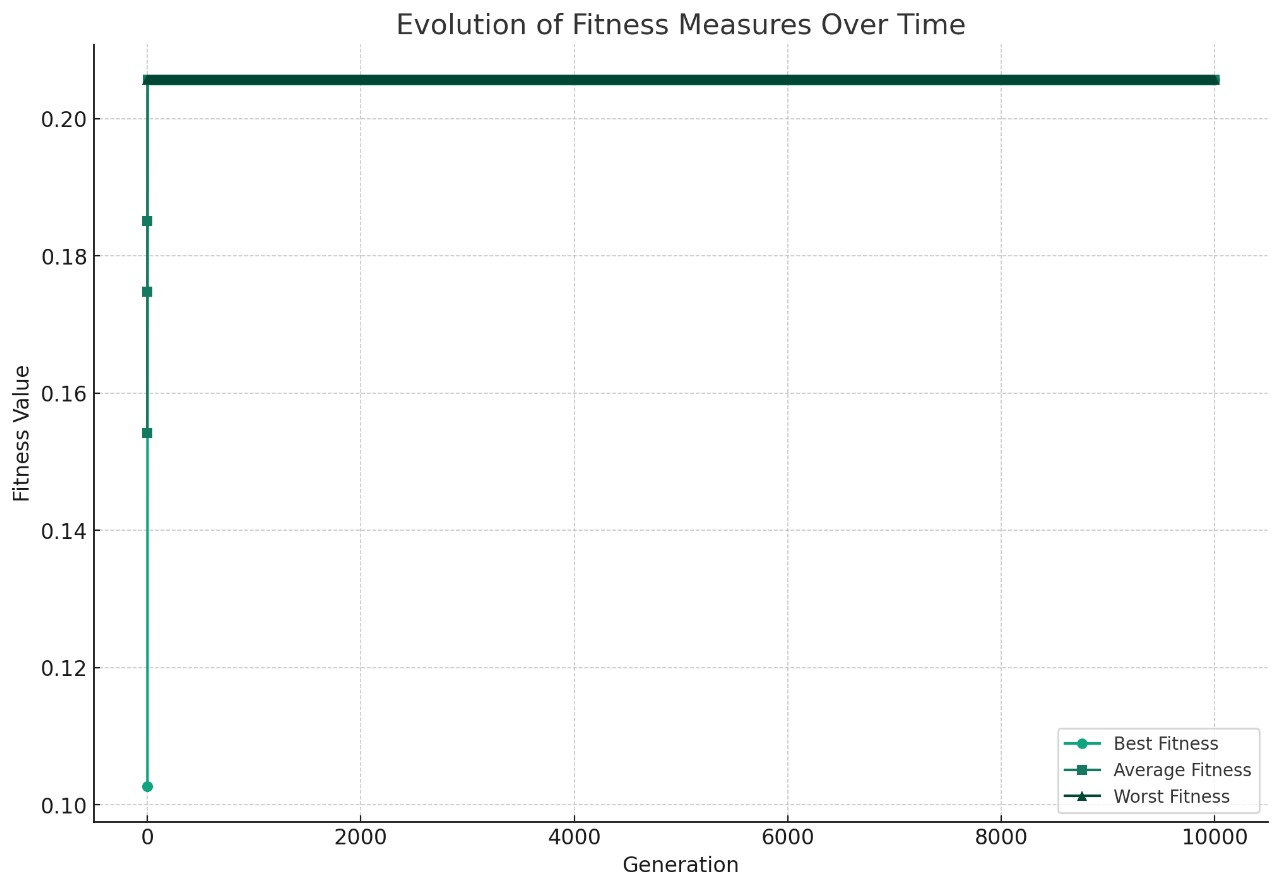
\includegraphics[width=0.5\linewidth]{1tentativa.png}
    \caption{Evolução da população com 10000 gerações}
    \label{fig:first-attempt}
\end{figure}

No teste seguinte a mudança  foi aplicada ao número de gerações com 200(2(\%da primeira tentativa) e obteve-se resultados melhores, porém com pouca informação para ser analisada.

\begin{figure}[h]
    \centering
    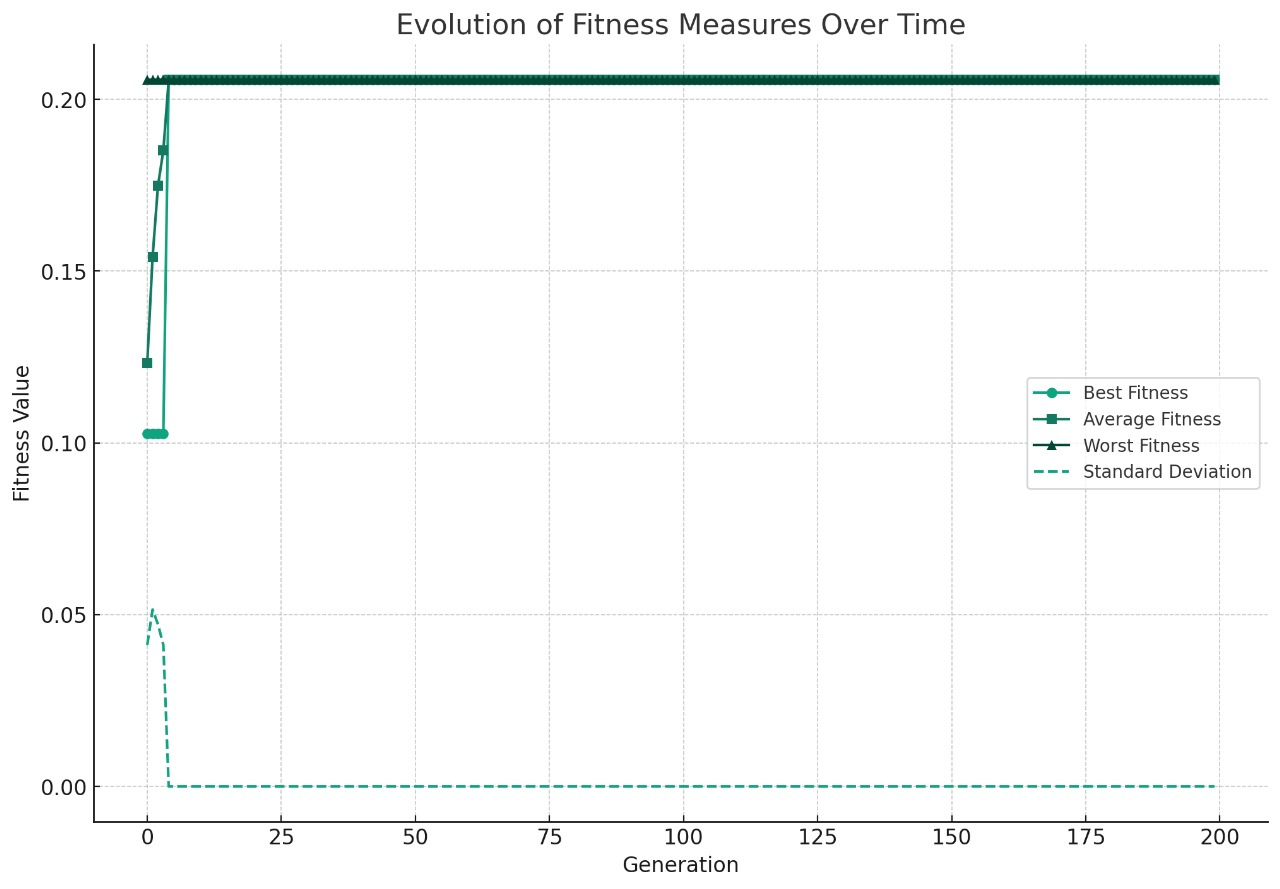
\includegraphics[width=0.5\linewidth]{2tentativa.png}
    \caption{Evolução da população com 200 gerações}
    \label{fig: second-attempt}
\end{figure}

Na terceira tentativa, ambos número de gerações e número de da população foram mudadas para 100, e com isso resultados mais satisfatórios foram apresentados.

\begin{figure}[H]
    \centering
    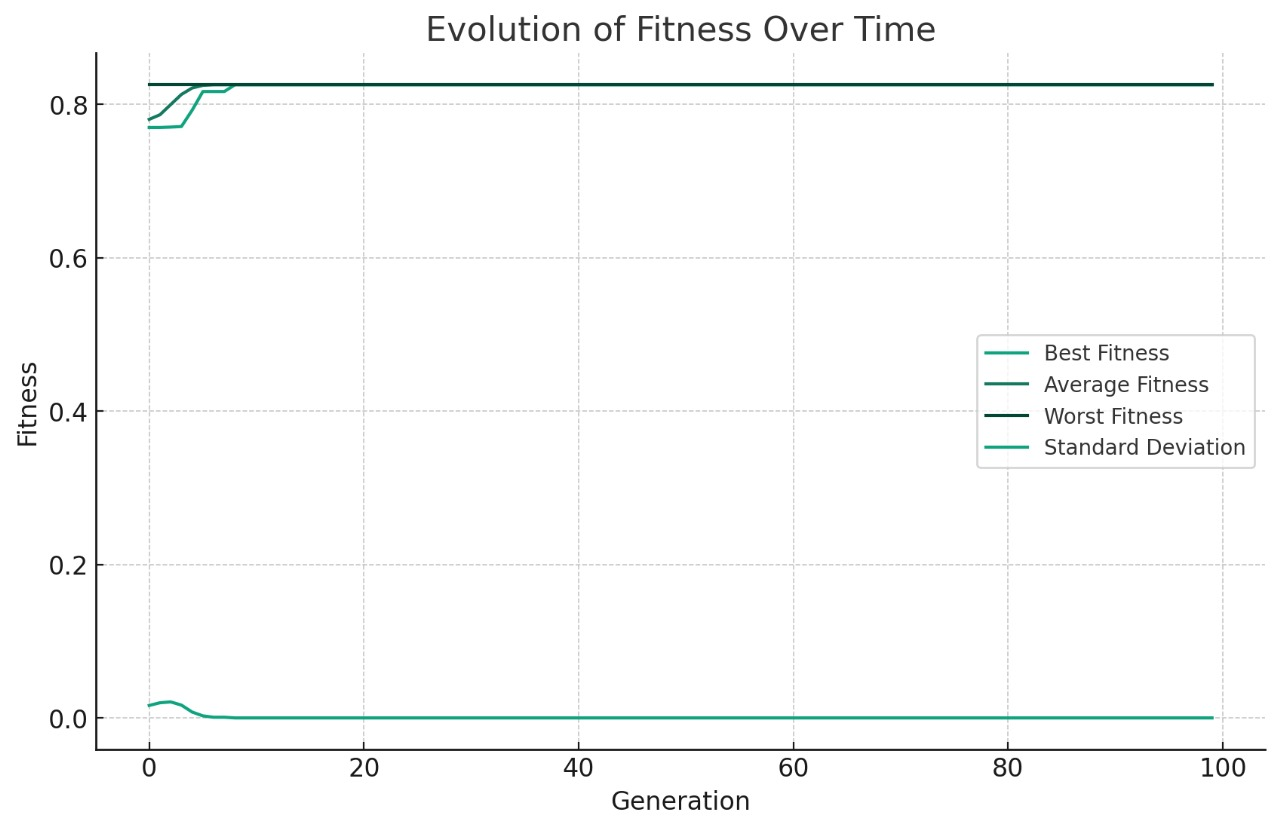
\includegraphics[width=0.5\linewidth]{3tentativa.png}
    \caption{Evolução da população com 100 gerações e 100 indivíduos}
    \label{fig:third-attempt}
\end{figure}

Na última tentativa com a população agora com o tamanho de 1000, o tempo de processamento aumentou significativamente porém os resultados quase não mudaram. Com um desvio padrão de aproximadamente de 0.01 e fitness entre 0.76 e 0.84

\begin{figure}[h]
    \centering
    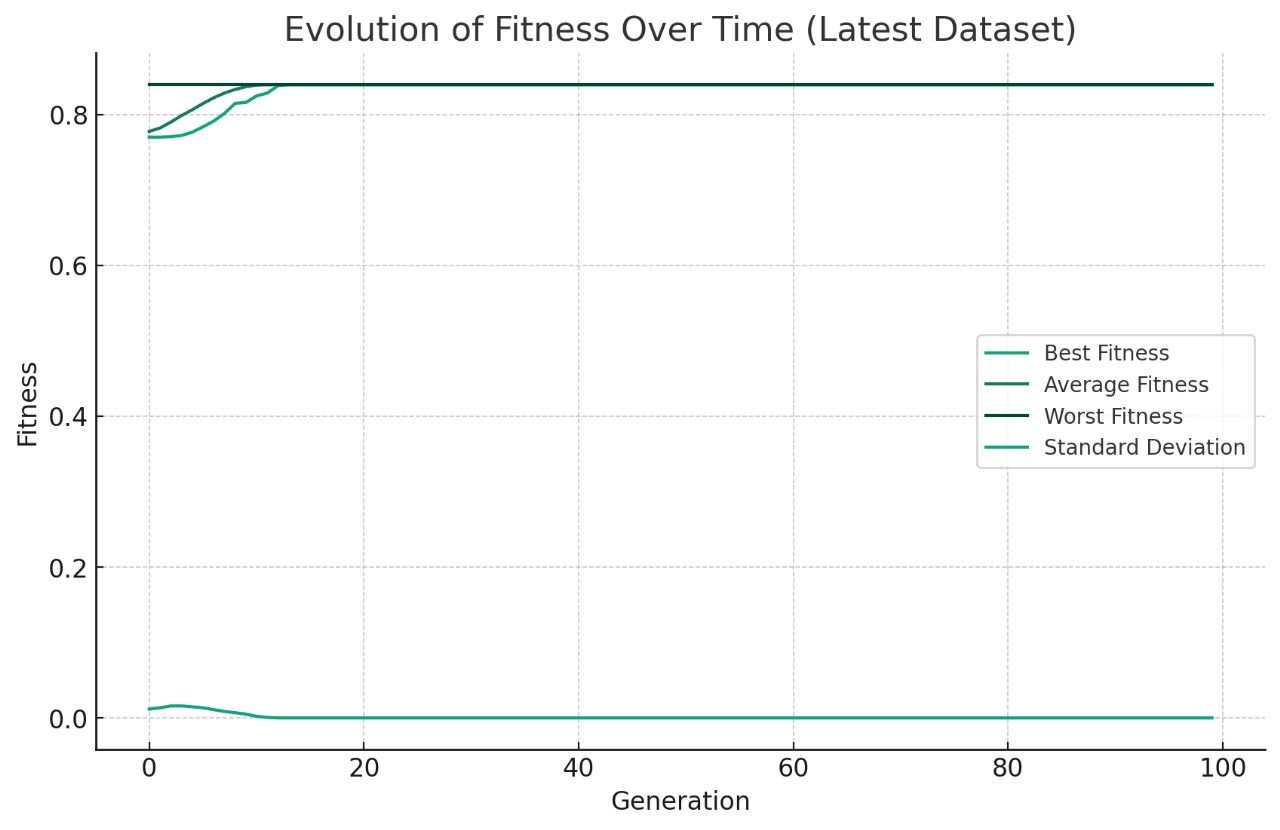
\includegraphics[width=0.5\linewidth]{4tentativa.png}
    \caption{Evolução da população com 100 gerações e 1000 indivíduos}
    \label{fig:fourth-attempt}
\end{figure}

\subsection{Resultados na abordagem sexuada}

\section{Conclusões e Trabalhos Futuros}
Afim de diminuir as consequências negativas de incêndios e em conclusão do que foi escrito nesse papel, dado que entre os fatores que foram analisados há três tipo de vegatação, três estados de propragação do fogo, a umidade do ar.
Depois de todos os testes o resultado final obtido foi com a população com tamanho 1000 e 100 iterações, porém com aproximadamente apenas 16 iterações resultou num ótimo de aproximadamente 0.99, o que significa que o algoritmo proposto teve 99\% de compatibilidade com a simulação real, resultado notável para auxiliar no combates a incêndios.

% TODO para Seiji/Maca:
% Falar na conclusão sobre a taxa de elitismo reversa, não vou colocar agora pq acho melhor esperar vcs melhorarem a parte de resultados e discussão

Em trabalhos futuros será testado a influência da variação do $\alpha$ no crossover BLX-$\alpha$ e a influência da taxa de mutação na abordagem assexuada, além de testar a influência do tamanho da população e do número de gerações.

\section{References}


\bibliographystyle{sbc}
\bibliography{mybib}

\end{document}
